\chapter{STUDI LITERATUR}
\label{chap:studi-literatur}
\section{Hoaks dan Tantangan Kualitas Informasi di Era Digital}
Perkembangan ekosistem digital telah mempermudah produksi dan distribusi informasi dalam skala yang jauh lebih besar dibandingkan sebelumnya. 
Kemudahan ini membawa manfaat, tetapi juga membuka ruang yang luas bagi munculnya hoaks. 
\textcite{emilremus2025} menjelaskan bahwa \textit{fake news} berkembang sebagai konsekuensi dari arus informasi yang tidak terkendali, 
lemahnya mekanisme verifikasi, serta perubahan pola konsumsi informasi masyarakat. Dalam lingkungan digital yang lebih mengutamakan kecepatan, 
banyak pengguna membagikan informasi tanpa melakukan pengecekan terlebih dahulu. 
Situasi ini memungkinkan konten palsu menyebar ke ribuan pengguna dalam waktu yang sangat singkat.

Hoaks tidak hanya berbentuk klaim palsu secara langsung. \textcite{emilremus2025} menunjukkan bahwa fenomena ini mencakup spektrum yang lebih luas, mulai dari misinformasi—informasi salah yang disebarkan tanpa niat menipu—hingga disinformasi yang diproduksi secara sengaja untuk memberikan kesan yang menyesatkan. Ada pula mal-informasi, satire, serta manipulasi konten berbasis gambar atau video. Beragamnya bentuk dan gaya penyajian membuat proses identifikasi hoaks semakin rumit karena setiap jenis memiliki pola penyebaran, tujuan, dan dampak yang berbeda.

Tantangan kualitas informasi juga berkaitan erat dengan siapa yang menyebarkannya. Berdasarkan analisis \textcite{emilremus2025}, terdapat dua kelompok utama yang berperan dalam memperluas jangkauan hoaks. Kelompok pertama adalah aktor jahat yang secara sengaja memproduksi dan mendistribusikan konten palsu, termasuk bot, akun anonim, atau operasi informasi yang terorganisasi. Kelompok kedua adalah pengguna biasa yang secara tidak sadar ikut menyebarkan hoaks karena rendahnya literasi digital, kecenderungan untuk mempercayai informasi yang sesuai dengan pandangan pribadi, atau dorongan emosional saat melihat konten tertentu. Kedua kelompok ini mempercepat rantai penyebaran hoaks dan membuat penanganannya semakin kompleks.

Selain faktor perilaku pengguna, dinamika penyebaran konten di media sosial turut memperburuk kondisi kualitas informasi. \textcite{alghamdi2024comprehensive} mencatat bahwa yang membuat hoaks sangat mudah viral adalah kecenderungan algoritma untuk mendorong konten yang bersifat sensasional atau emosional. Hal ini dapat meningkatkan polarisasi politik, menyebarkan misinformasi kesehatan, dan memperlemah kepercayaan publik terhadap institusi resmi. Dalam banyak kasus, informasi palsu yang menarik perhatian lebih cepat diterima dan dibagikan oleh pengguna dibandingkan informasi faktual yang biasanya memiliki gaya penyajian yang lebih formal dan kurang menarik secara emosional.

Dilihat dari sisi teknis juga tantangan dalam mendeteksi dan memverifikasi hoaks semakin meningkat. \textcite{emilremus2025} menyoroti bahwa volume data yang sangat besar, keberagaman \textit{platform}, serta hadirnya konten multimodal seperti gambar editan, video manipulatif, dan \textit{deepfake} membuat proses verifikasi manual tidak lagi memadai. Sementara itu, \textcite{alghamdi2024comprehensive} menekankan bahwa sistem verifikasi manusia tidak mampu mengimbangi kecepatan penyebaran informasi di media sosial, sehingga banyak konten penting sudah terlanjur viral sebelum sempat diverifikasi oleh lembaga pemeriksa fakta. Ketidakseragaman struktur data, minimnya anotasi, dan variasi konteks membuat verifikasi otomatis pun menghadapi tantangan tersendiri.

Maka dari itu, ini menunjukkan bahwa sebenarnya tantangan kualitas informasi di era digital saat ini tidak hanya disebabkan oleh karakteristik konten yang semakin kompleks, tetapi juga dari perilaku pengguna, mekanisme algoritma \textit{platform}, dan keterbatasan teknologi verifikasi. Tantangan ini menuntut pendekatan multidisipliner yang melibatkan pemahaman mengenai faktor-faktor yang ada, mulai dari faktor sosial, teknis, perilaku, serta peran \textit{platform} dalam mengatur arus informasi. Pemahaman ini yang menjadi dasar penting serta alasan bagi penelitian teknis seperti tugas akhir ini, yang berupaya menganalisis dan mengevaluasi model deteksi hoaks berbasis \textit{machine learning} untuk mendukung kualitas informasi yang lebih aman dan terpercaya.


\section{Pendekatan Deteksi Hoaks (ML Klasik, DL, dan LLM)}

Penelitian mengenai deteksi hoaks telah berkembang melalui berbagai pendekatan yang memiliki fokus analisis berbeda. Secara umum, pendekatan tersebut dapat dipetakan menjadi tiga kategori utama berdasarkan tinjauan \textcite{alghamdi2024comprehensive}, yaitu berbasis konten, berbasis konteks atau pola penyebaran, dan pendekatan hibrida. Ketiganya berkembang sebagai respons terhadap kebutuhan untuk memahami tidak hanya bagaimana sebuah berita ditulis, tetapi juga bagaimana ia disebarkan serta siapa yang memproduksinya. Kerangka ini menjadi dasar untuk memahami posisi pendekatan yang digunakan dalam penelitian ini.

Pendekatan berbasis konten merupakan metode yang menganalisis karakteristik linguistik dari teks berita. \textcite{alghamdi2024comprehensive} menjelaskan bahwa berita hoaks sering kali menggunakan bahasa yang lebih emosional, subjektif, repetitif, dan memiliki struktur kalimat yang cenderung sederhana. Fitur seperti frekuensi kata, kosakata provokatif, tanda baca berlebihan, hingga pola kapitalisasi tertentu dapat menjadi indikator penting bagi model klasifikasi. Pendekatan ini banyak dipakai karena tidak membutuhkan informasi tambahan seperti pola interaksi pengguna dalam jaringan sosial. Selain itu, pendekatan ini efektif untuk deteksi dini, terutama ketika hanya teks yang tersedia. Penelitian ini juga menggunakan metode berbasis konten karena \textit{dataset} berbahasa Indonesia yang digunakan sebagian besar hanya memuat teks berita.

Selain konten, beberapa penelitian mengusulkan pendekatan berbasis konteks atau penyebaran dengan memanfaatkan pola interaksi pengguna, struktur penyebaran informasi, dan dinamika percakapan di media sosial. Contohnya meliputi analisis \textit{engagement} seperti retweet, komentar, atau jaringan percakapan yang dibentuk oleh para pengguna. Pendekatan ini memungkinkan model mendeteksi hoaks berdasarkan pola penyebaran yang tidak biasa atau adanya kemungkinan operasi yang terkoordinasi. Pada banyak studi, pendekatan ini dikembangkan melalui Graph Neural Networks (GNN) yang memodelkan interaksi antar pengguna dan pola distribusi konten. Namun pendekatan tersebut hanya dapat diterapkan apabila tersedia data penyebaran yang lengkap, sesuatu yang tidak relevan untuk \textit{dataset} berita yang digunakan dalam penelitian ini.

Pendekatan ketiga adalah pendekatan hibrida yang menggabungkan analisis konten, informasi konteks, dan metadata sumber untuk menghasilkan prediksi yang lebih komprehensif. \textcite{emilremus2025} menunjukkan bahwa perkembangan terbaru dalam deteksi hoaks semakin mengarah pada penggunaan metadata seperti domain situs, kredibilitas media, waktu publikasi, dan informasi tambahan lainnya. Pendekatan ini memberikan gambaran yang lebih utuh mengenai kredibilitas suatu berita, meskipun kompleksitasnya lebih tinggi dibandingkan metode berbasis konten saja. Penelitian ini memanfaatkan versi ringan dari pendekatan hibrida dengan menambahkan fitur sumber sederhana seperti domain atau jenis media, sembari mempertahankan fokus utama pada analisis konten.

Seiring dengan beragamnya pendekatan tersebut, metode komputasi untuk deteksi hoaks juga mengalami perkembangan signifikan. Teknik pertama yang banyak digunakan adalah \textit{machine learning} klasik seperti Na\"{\i}ve Bayes, Support Vector Machine, dan Random Forest. \textcite{Alghamdi2022info13120576} menegaskan bahwa ketiga algoritma ini memiliki sejumlah keunggulan seperti kebutuhan komputasi yang rendah, interpretabilitas yang baik, serta performa yang stabil pada \textit{dataset} berukuran sedang. SVM dikenal efektif untuk data berdimensi tinggi, Na\"{\i}ve Bayes sederhana tetapi kuat untuk teks pendek, sedangkan Random Forest unggul dalam stabilitas melalui pendekatan \textit{ensemble}. Meskipun demikian, metode ini membutuhkan rekayasa fitur manual dan sering kali tidak dapat menangkap hubungan semantik yang lebih kompleks dalam teks panjang.

Perkembangan berikutnya adalah penggunaan \textit{deep learning}, termasuk CNN, RNN, LSTM, serta model transformer seperti BERT. Model-model ini mampu mengenali pola konteks jangka panjang dalam teks dan menangkap makna bahasa secara lebih mendalam. \textcite{emilremus2025} menyoroti bahwa model berbasis transformer menjadi sangat dominan karena mampu mempelajari hubungan antar kata dalam satu kalimat secara lebih efektif dibandingkan metode tradisional. Studi \textcite{pekandi2025evaluating} menunjukkan bahwa IndoBERT—model transformer yang dilatih khusus pada bahasa Indonesia—mampu mencapai akurasi hingga 92 persen untuk deteksi hoaks, melampaui model CNN-LSTM dan \textit{ensemble} machine learning klasik. Meskipun demikian, model-model \textit{deep learning} membutuhkan \textit{dataset} besar, sumber daya komputasi tinggi, serta proses pelatihan yang lebih kompleks.

Perkembangan paling mutakhir dalam deteksi hoaks adalah penggunaan \textit{large language models} (LLM). \textcite{emilremus2025} menjelaskan bahwa LLM seperti GPT, LLaMA, atau Gemini memiliki kemampuan menganalisis teks dengan pemahaman konteks yang lebih luas, menghasilkan data tambahan, merangkum informasi, atau melakukan penalaran berbasis pengetahuan eksternal. Meskipun memiliki potensi besar, penggunaan LLM juga menghadapi tantangan seperti biaya komputasi yang tinggi, risiko halusinasi, serta kebutuhan evaluasi yang ketat untuk memastikan keandalan prediksi.

Dengan memahami seluruh peta pendekatan tersebut, Tugas Akhir ini menempatkan dirinya sebagai studi berbasis konten yang menggunakan algoritma \textit{machine learning} klasik dengan eksplorasi terbatas pada metadata sumber. Pemilihan pendekatan ini didasarkan pada karakteristik \textit{dataset}, kebutuhan efisiensi, serta relevansinya sebagai \textit{baseline} yang kokoh untuk penelitian lanjutan. Selain itu, batasan ruang lingkup tugas akhir membuat pendekatan berbasis ML klasik menjadi pilihan yang realistis dan sesuai dengan tujuan Tugas Akhir, sementara model \textit{deep learning} atau transformer ditempatkan sebagai peluang pengembangan pada tahap berikutnya.


\section{\textit{Preprocessing} Teks Bahasa Indonesia dan Representasi TF-IDF}
\par TF-IDF (Term Frequency-Inverse Document Frequency) merupakan metode representasi teks yang paling umum digunakan dalam klasifikasi dokumen. Metode ini menghitung bobot suatu kata dalam sebuah dokumen berdasarkan seberapa sering kata tersebut muncul di dokumen tertentu, dan seberapa jarang kata tersebut muncul di seluruh korpus. TF-IDF efektif dalam menghilangkan kata-kata umum (seperti “yang”, “adalah”, “itu”) dan menonjolkan kata-kata penting yang menjadi penanda topik sebuah berita.

\par Beberapa penelitian telah membuktikan bahwa TF-IDF sangat efektif dalam meningkatkan akurasi model klasifikasi berita hoaks. \textcite{prasetyo2019evaluation} mengevaluasi penggunaan TF-IDF pada klasifikasi berita hoaks Indonesia dan menemukan bahwa representasi TF-IDF secara signifikan meningkatkan akurasi model berbasis Naïve Bayes dan SVM. Temuan serupa juga dilaporkan oleh \textcite{prasetijo2017hoax}, yang menggabungkan TF-IDF dengan SVM dan SGD untuk mendeteksi hoaks dan mencapai akurasi sekitar 86\%.

\subsection{\textit{Preprocessing} Teks Bahasa Indonesia}

\begin{figure}[h!] % pilihan opsi yang disarankan: t = top, b = bottom, h = here
	\centering
  \captionsetup{justification=centering}
    	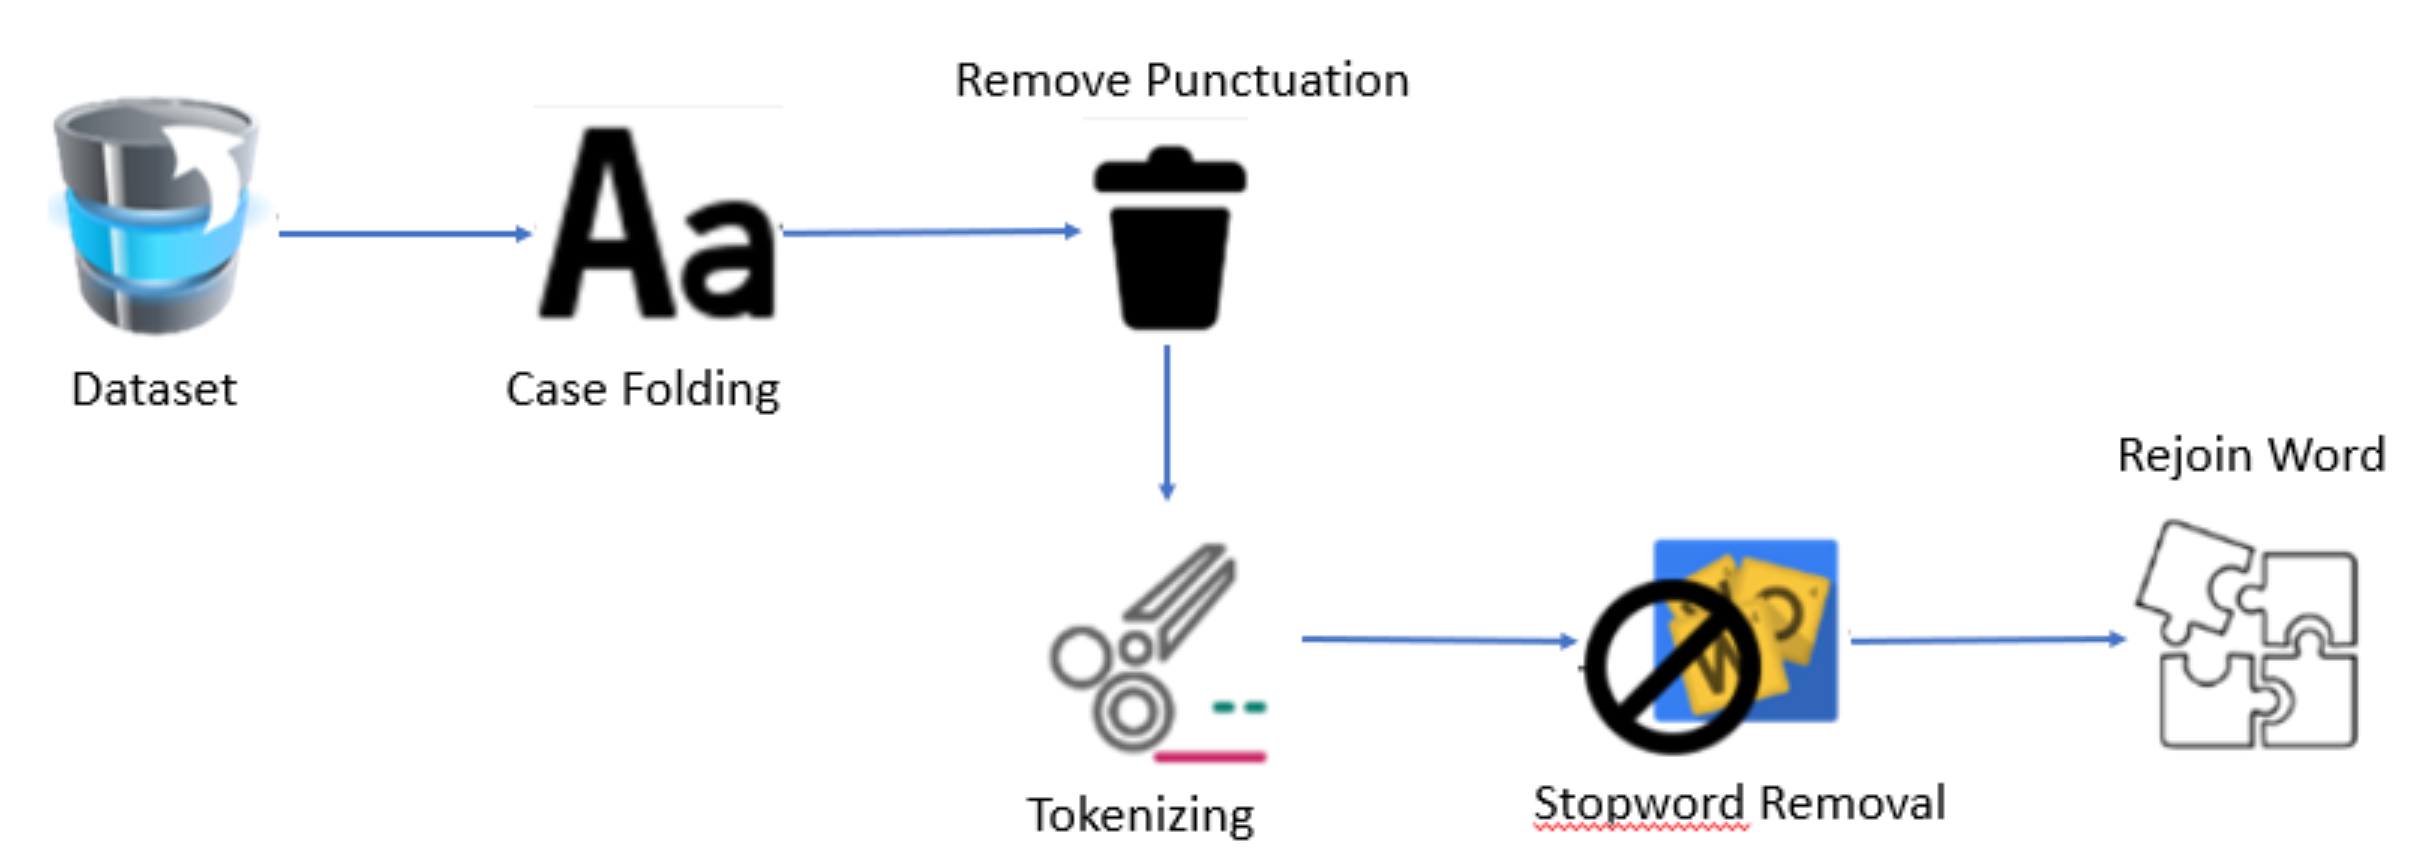
\includegraphics[width=0.7\textwidth]{image/preprocessing-steps.png}
	\caption{\textit{Preprocessing steps}}
	\label{gambar:preprocessing}
\end{figure}

\textit{Preprocessing} merupakan langkah penting untuk menyiapkan teks agar dapat diproses oleh algoritma \textit{machine learning}. Pada penelitian deteksi hoaks berbahasa Indonesia, seperti yang dilakukan \textcite{pratiwi2022hoax}, dan tahapannya tertera pada Gambar \ref{gambar:preprocessing}.
tahapan ini akan mencakup \textit{case folding}, \textit{cleaning}, tokenisasi, \textit{stopword removal}, dan \textit{stemming}. Tujuannya adalah mengubah teks mentah yang tidak seragam menjadi bentuk yang lebih terstruktur dan konsisten sehingga fitur yang diekstraksi pada tahap berikutnya benar-benar mencerminkan isi dokumen.
\begin{enumerate}
	
	\item \textbf{Case folding}

	\textit{Case folding} adalah proses mengubah seluruh huruf dalam teks menjadi huruf kecil. Langkah sederhana ini mencegah model membedakan kata yang sama hanya karena perbedaan kapitalisasi, misalnya “Hoaks”, “hoaks”, dan “HOAKS”. Dengan case folding, ketiga bentuk tersebut dipandang sebagai satu token yang sama sehingga distribusi kata menjadi lebih stabil.\\

	\item \textbf{Cleaning}  

	\textit{Cleaning} bertujuan menghilangkan elemen teks yang tidak relevan untuk analisis isi. Pada tahap ini biasanya dihapus karakter non-alfabet, angka, tanda baca tertentu, URL, alamat email, hingga simbol atau emoji yang tidak diperlukan. Dalam konteks berita hoaks Indonesia, banyak teks yang mengandung tautan ke laman lain, tag media sosial, atau karakter khusus dari proses penyalinan. Pembersihan ini membantu mengurangi \textit{noise} sehingga model tidak terganggu oleh token yang tidak bermakna.\\

	\item \textbf{Tokenisasi}  

	Tokenisasi adalah proses memecah teks yang telah dibersihkan menjadi satuan kata (token). Tokenisasi biasanya dilakukan berdasarkan spasi atau tanda baca sehingga setiap kata menjadi unit analisis tersendiri. Misalnya, kalimat "Berita ini ternyata hoaks" akan dipecah menjadi token ["berita", "ini", "ternyata", "hoaks"].\\

	\item \textbf{Stopword removal}  

	\textit{Stopword removal} menghapus kata-kata yang sangat sering muncul tetapi tidak membantu membedakan dokumen. Kata seperti "yang", "adalah", "itu", "dan", atau "untuk" biasanya dimasukkan ke dalam daftar stopword bahasa Indonesia. Dengan menghilangkan kata-kata ini, model dapat lebih fokus pada kata yang membawa makna spesifik. \textcite{pratiwi2022hoax} juga menggunakan daftar stopword Indonesia sebagai bagian dari \textit{pipeline} \textit{preprocessing} mereka.\\

	\item \textbf{Stemming}  

	\textit{Stemming} mereduksi kata ke bentuk dasarnya. Bahasa Indonesia memiliki struktur morfologi yang kaya, sehingga algoritma seperti Nazief--Adriani atau pustaka Sastrawi banyak digunakan. Sebagai contoh, kata "mempunyai", "kepunyaan", dan "punya" akan distem menjadi bentuk dasar "punya". Dengan stemming, variasi kata yang berasal dari akar yang sama tidak dipandang sebagai token berbeda sehingga distribusi fitur menjadi lebih padat dan lebih mudah dipelajari oleh model.\\
\end{enumerate}

Rangkaian tahapan ini menjadi pola umum pada berbagai penelitian deteksi hoaks Indonesia dan terbukti meningkatkan kualitas representasi teks sebelum masuk ke tahap ekstraksi fitur.

\subsection{Representasi Fitur TF-IDF}

Setelah proses \textit{preprocessing} selesai, teks yang telah bersih dan terstruktur perlu diubah menjadi bentuk numerik agar dapat diproses oleh algoritma \textit{machine learning}. Salah satu metode yang paling banyak digunakan adalah \textit{Term Frequency-Inverse Document Frequency} (TF-IDF). Representasi ini memberikan bobot pada setiap kata berdasarkan frekuensi kemunculannya dalam dokumen dan seberapa jarang kata tersebut muncul di seluruh korpus.

\textbf{\textit{Term Frequency} (TF)}  

\textit{Term Frequency} mengukur frekuensi relatif kata $w$ dalam dokumen $d$. Rumus umum TF adalah:

\begin{align}
TF(w,d) = \frac{\text{count}(w \in d)}{\text{total kata pada } d} \label{eq=rumus-tf}
\end{align}
Keterangan:  
$w$ = kata tertentu,  
$d$ = dokumen,  
$\text{count}(w \in d)$ = jumlah kemunculan kata $w$ dalam dokumen.

\textbf{\textit{Inverse Document Frequency} (IDF)}  

IDF mengukur seberapa jarang kata muncul dalam korpus. Rumus IDF dicatat dalam bentuk:

\begin{align}
IDF(w) = \log \left( \frac{N}{df(w)} \right) \label{eq=rumus-idf}
\end{align}
Keterangan:  
$N$ = jumlah total dokumen,  
$df(w)$ = jumlah dokumen yang mengandung kata $w$.

\textbf{Bobot TF-IDF}  

Bobot TF-IDF diperoleh dengan mengalikan TF dan IDF:
\begin{align}
TFIDF(w,d) = TF(w,d) \times IDF(w) \label{eq=rumus-tfidf}
\end{align}

Nilai TF-IDF akan tinggi ketika sebuah kata sering muncul pada satu dokumen, tetapi jarang muncul di dokumen lain. Kondisi ini menunjukkan bahwa kata tersebut memiliki daya diskriminasi tinggi dan penting untuk membedakan dokumen. Sebaliknya, kata yang muncul di hampir semua dokumen akan memiliki nilai TF-IDF rendah karena dianggap kurang informatif. Dengan cara ini, setiap dokumen direpresentasikan sebagai vektor berdimensi tinggi yang berisi bobot TF-IDF untuk setiap kata yang dipertahankan setelah \textit{preprocessing}.

Berbagai penelitian deteksi hoaks Indonesia seperti \textcite{prasetyo2019evaluation}, \textcite{pratiwi2022hoax}, dan \textcite{sihombing2020article} menunjukkan bahwa representasi TF-IDF memberikan performa stabil dan efektif ketika dipadukan dengan algoritma \textit{machine learning} klasik seperti Na\"{\i}ve Bayes dan SVM. Hal ini menjadi salah satu alasan utama penggunaan TF-IDF dalam tugas akhir ini.

\subsection{Justifikasi Penggunaan Representasi TF-IDF}

Pemilihan TF-IDF sebagai metode representasi teks dalam penelitian ini didasarkan pada pertimbangan metodologis dan bukti empiris dari berbagai penelitian deteksi hoaks berbahasa Indonesia. TF-IDF menawarkan pendekatan yang sederhana namun efektif untuk menonjolkan kata yang memiliki nilai diskriminatif tinggi dalam suatu dokumen. Representasi ini memberikan bobot lebih besar pada kata yang sering muncul dalam satu teks tetapi jarang ditemukan pada teks lain dalam korpus. Dengan cara ini, model dapat lebih mudah membedakan pola bahasa antara berita hoaks dan non-hoaks. Kesederhanaan struktur TF-IDF juga menjadikannya lebih mudah diinterpretasikan dibandingkan representasi lain, sehingga sesuai untuk penelitian yang memfokuskan diri pada algoritma \textit{machine learning} klasik dan kebutuhan evaluasi yang transparan.

Alternatif representasi seperti Word2Vec dan GloVe mampu menangkap hubungan semantik antarkata melalui vektor kontinu, sementara \textit{embedding} kontekstual seperti BERT atau IndoBERT memberikan representasi yang jauh lebih kaya. Namun pendekatan tersebut membutuhkan proses pelatihan tambahan, sumber daya komputasi lebih besar, serta kompleksitas dalam pengaturan hiperparameter. Dalam konteks tugas akhir ini yang menggunakan \textit{dataset} berukuran sedang dan berfokus pada perbandingan tiga algoritma klasik, penggunaan \textit{embedding} canggih tidak sejalan dengan batasan ruang lingkup Tugas Akhir. Selain itu, penggunaan representasi yang lebih kompleks dapat memengaruhi interpretabilitas hasil, terutama ketika tujuan Tugas Akhir mencakup penyediaan \textit{baseline} yang stabil untuk penelitian lanjutan.

Efektivitas TF-IDF dalam deteksi hoaks bahasa Indonesia juga didukung oleh hasil empiris dari berbagai penelitian sebelumnya. \textcite{prasetyo2019evaluation} menunjukkan bahwa penggunaan TF-IDF secara konsisten meningkatkan akurasi model Na\"{\i}ve Bayes dan SVM dalam mengklasifikasikan berita hoaks. Penelitian \textcite{sihombing2020article} menemukan bahwa kombinasi TF-IDF dan SVM mampu mencapai akurasi lebih dari 90 persen pada \textit{dataset} berita daring Indonesia. Hasil serupa terlihat pada penelitian \textcite{pratiwi2022hoax} yang menggunakan TF-IDF untuk memetakan fitur teks pada \textit{dataset} berita hoaks berbahasa Indonesia, serta penelitian lain seperti \textcite{prasetijo2017hoax} dan \textcite{triyono2023indonesian}, yang memperlihatkan stabilitas performa TF-IDF dalam berbagai model \textit{machine learning} klasik. Konsistensi ini memperkuat justifikasi bahwa TF-IDF merupakan representasi yang tidak hanya efisien, tetapi juga mampu memberikan hasil kompetitif pada berbagai \textit{dataset} hoaks Indonesia.

Berdasarkan pertimbangan tersebut, TF-IDF menjadi pilihan yang paling relevan untuk Tugas Akhir ini. Metode ini mendukung kebutuhan analisis yang efisien, dapat diinterpretasikan, dan sejalan dengan pendekatan \textit{machine learning} klasik yang digunakan. Penggunaan TF-IDF juga memastikan bahwa hasil Tugas Akhir dapat dibandingkan secara langsung dengan studi terdahulu sehingga memberikan dasar yang kuat bagi pengembangan model deteksi hoaks pada tahap selanjutnya.

\subsection{Representasi Fitur Sumber dengan One-Hot \textit{encoding}}
Pemanfaatan fitur sumber dalam Tugas Akhir ini berangkat dari asumsi bahwa pola hoaks tidak hanya muncul pada isi teks, tetapi juga dapat dipengaruhi oleh karakteristik asal berita, seperti domain situs atau jenis media tempat artikel dipublikasikan. Informasi tersebut bersifat kategorikal dan tidak dapat langsung digunakan sebagai masukan bagi algoritma klasifikasi yang mengharuskan representasi numerik. Oleh karena itu, diperlukan proses \textit{encoding} agar fitur sumber dapat diperlakukan sebagai bagian dari vektor fitur yang diproses oleh model.

Penelitian \textcite{herdian2024studi} tersebut menguji dua teknik \textit{encoding} utama yang lazim digunakan pada data kategorikal. Label \textit{encoding} merepresentasikan setiap kategori sebagai bilangan integer yang berbeda, namun cara ini secara implisit menimbulkan hubungan ordinal antar kategori meskipun dalam kenyataannya kategori tersebut tidak memiliki urutan. Sebaliknya, one-hot \textit{encoding} menghasilkan vektor biner untuk setiap kategori dan tidak mengasumsikan adanya hubungan berjenjang antar nilai kategorikal. Pendekatan ini umumnya lebih aman untuk variabel nominal karena tidak memperkenalkan struktur matematis yang tidak sesuai dengan makna datanya.

Hasil penelitian \textcite{herdian2024studi} menunjukkan bahwa pemilihan teknik \textit{encoding} berpengaruh terhadap performa model. One-hot \textit{encoding} menghasilkan nilai R-squared 0.85, jauh lebih tinggi dibanding label \textit{encoding} yang hanya mencapai 0.54, sehingga model yang memanfaatkan one-hot \textit{encoding} mampu merepresentasikan data kategorikal dengan lebih tepat dalam konteks pemodelan yang mereka bangun . Temuan ini menguatkan prinsip umum dalam \textit{Feature Enigneering} bahwa variabel kategorikal nominal sebaiknya direpresentasikan dengan \textit{encoding} yang tidak menambahkan asumsi hierarki antar kategori.

Dalam konteks Tugas Akhir deteksi hoaks ini, fitur sumber seperti domain situs atau kategori media memiliki sifat nominal dan jumlah kategorinya relatif terbatas setelah proses pemetaan. Berdasarkan pertimbangan tersebut serta temuan dari studi sebelumnya, penelitian ini menggunakan \textit{one-hot} \textit{encoding} untuk merepresentasikan fitur sumber. Teknik ini memungkinkan model memanfaatkan informasi sumber tanpa menambahkan struktur numerik yang tidak relevan. Selain itu, fitur seperti nama penulis tidak dimasukkan karena jumlah kategorinya sangat besar dan berpotensi menambah noise tanpa kontribusi signifikan terhadap akurasi model.

\section{Algoritma Na\"{\i}ve Bayes, SVM, dan Random Forest untuk Klasifikasi Teks}

\subsection{Na\"{\i}ve Bayes}

Na\"{\i}ve Bayes merupakan salah satu algoritma klasifikasi yang banyak digunakan dalam analisis teks karena kesederhanaan dan performanya yang stabil pada data berdimensi tinggi. Secara teoritis, model ini didasarkan pada Teorema Bayes yang memodelkan probabilitas posterior suatu kelas $C$ terhadap dokumen teks $d$. Teorema Bayes secara umum dirumuskan sebagai:
\begin{align}
P(C \mid d) = \frac{P(d \mid C)\, P(C)}{P(d)} \label{eq=teorema-bayes}
\end{align}
Keterangan:
$P(C \mid d)$ = probabilitas posterior kelas $C$ diberikan dokumen $d$,  
$P(d \mid C)$ = probabilitas likelihood dokumen $d$ diberikan kelas $C$,  
$P(C)$ = probabilitas prior kelas $C$,

Dalam konteks klasifikasi teks, dokumen direpresentasikan sebagai sekumpulan kata sehingga probabilitas dokumen diberikan kelas diturunkan dari probabilitas kemunculan kata-kata tersebut dalam kelas. Na\"{\i}ve Bayes menggunakan asumsi independensi antarf fitur, yaitu setiap kata dianggap tidak saling bergantung satu sama lain apabila kelasnya diketahui. Meskipun asumsi ini tidak sepenuhnya realistis untuk bahasa natural, berbagai penelitian menunjukkan bahwa model ini tetap efektif, sehingga sering disebut sebagai "na\"{\i}ve yet effective".

Varian Na\"{\i}ve Bayes yang paling umum digunakan untuk teks adalah \textit{Multinomial Na\"{\i}ve Bayes}, yang menghitung probabilitas berdasarkan frekuensi kemunculan kata dalam dokumen. Rumus prediksi kelas pada varian ini dapat dituliskan sebagai:
\begin{align}
% P(d \mid C) = \prod_{i=1}^{n} P(w_i \mid C)
P(C \mid d) \propto P(C) \prod_{i=1}^{n} P(w_i \mid C) \label{eq=rumus-Multinomial-NB}
\end{align}

dengan $w_i$ adalah kata ke-$i$ dalam dokumen. Pada tahap pelatihan, model menghitung probabilitas prior kelas berdasarkan distribusi kelas dan probabilitas bersyarat $P(w_i \mid C)$ dari frekuensi kata pada kelas tersebut. Pada tahap prediksi, probabilitas posterior dihitung untuk setiap kelas, dan kelas dengan nilai tertinggi dipilih sebagai hasil klasifikasi.

Keunggulan Na\"{\i}ve Bayes terletak pada kesederhanaan dan efisiensi komputasinya. Waktu pelatihan bersifat linear terhadap jumlah fitur, sehingga sangat sesuai untuk data teks yang \textit{sparse} dengan jumlah fitur besar. Selain itu, probabilitas kata yang dihasilkan memberikan interpretabilitas yang baik, memungkinkan peneliti mengidentifikasi kata yang paling berpengaruh terhadap prediksi model. Algoritma ini juga memiliki jumlah hiperparameter yang minimal sehingga cocok digunakan sebagai \textit{baseline} sebelum mencoba model yang lebih kompleks. 

Namun demikian, Na\"{\i}ve Bayes memiliki keterbatasan, seperti asumsi independensi kata yang membuat model kurang mampu menangkap hubungan semantik antar kata. Model ini juga cenderung kalah performa dibandingkan algoritma lain seperti SVM atau Random Forest pada data dengan pola bahasa yang lebih kompleks. Selain itu, terdapat risiko \textit{zero probability} ketika suatu kata tidak pernah muncul pada kelas tertentu, yang umumnya diatasi menggunakan teknik smoothing seperti \textit{Laplace smoothing}.

Dalam konteks deteksi hoaks berbahasa Indonesia, Na\"{\i}ve Bayes tetap relevan karena hoaks sering menampilkan pola linguistik yang khas, seperti penggunaan kata-kata emosional dan struktur kalimat yang sederhana. \textcite{pratiwi2022hoax} menunjukkan bahwa Multinomial Na\"{\i}ve Bayes yang dipadukan dengan TF-IDF mampu mencapai akurasi sekitar 71\% dengan nilai \textit{precision}, \textit{recall}, dan F1-score di atas 70\% pada \textit{dataset} berita hoaks Indonesia. Studi lain oleh \textcite{cahyono2024fast} juga melaporkan bahwa model berbasis Na\"{\i}ve Bayes bekerja efisien dalam mendeteksi hoaks terkait COVID-19 pada media sosial, terutama dalam kondisi yang membutuhkan prediksi cepat. Penelitian \textcite{prasetyo2019evaluation} turut menunjukkan bahwa penggunaan TF-IDF mampu meningkatkan performa Na\"{\i}ve Bayes secara signifikan pada klasifikasi hoaks Indonesia.

Berbagai pengembangan Na\"{\i}ve Bayes juga telah dilakukan untuk meningkatkan performanya. Varian \textit{Complement Na\"{\i}ve Bayes} dirancang untuk menangani ketidakseimbangan kelas yang sering muncul pada \textit{dataset} hoaks, sedangkan \textit{Bernoulli Na\"{\i}ve Bayes} digunakan ketika fitur direpresentasikan dalam bentuk biner. Namun, untuk tugas akhir ini, Multinomial Na\"{\i}ve Bayes dipilih karena paling sesuai dengan representasi fitur TF-IDF dan karakteristik data teks berita yang berbasis frekuensi kata.

\subsection{Support Vector Machine (SVM)}

Support Vector Machine (SVM) merupakan salah satu algoritma yang banyak digunakan untuk tugas klasifikasi teks karena kemampuannya menemukan batas pemisah yang optimal antara dua kelas dalam ruang fitur berdimensi tinggi. Intuisi dasar SVM adalah mencari sebuah \textit{hyperplane} yang dapat memisahkan data dengan margin terbesar, yaitu jarak antara \textit{hyperplane} dan titik-titik terdekat dari masing-masing kelas. Dalam representasi TF-IDF yang digunakan pada Tugas Akhir ini, setiap dokumen diproyeksikan ke ruang fitur berukuran sangat besar, sering kali mencapai ribuan dimensi. Karakteristik ini sesuai dengan SVM karena algoritma ini dirancang untuk bekerja optimal pada data \textit{sparse} berdimensi tinggi.

Formulasi dasar SVM untuk kasus linear dapat dinyatakan sebagai permasalahan optimisasi untuk meminimalkan norma vektor bobot. Tujuannya adalah memperoleh \textit{hyperplane} dengan margin maksimum:
\begin{align}
\min \frac{1}{2} \lVert w \rVert^2 \label{eq=rumus-svm}
\end{align}
dengan constraint:
\begin{align}
y_i (w \cdot x_i + b) \ge 1,\quad \forall i = 1, \ldots, n \label{eq=rumus-constraint-svm}
\end{align}

dengan $w$ sebagai vektor normal hyperplane, $b$ adalah bias, $x_i$ adalah vektor fitur dokumen, dan $y_i$ merupakan label kelas.

Ketika data tidak dapat dipisahkan secara sempurna, SVM menggunakan pendekatan \textit{soft margin} dengan menambahkan variabel slack $\xi_i$ dan parameter regularisasi $C$ untuk mengontrol keseimbangan antara margin dan kesalahan klasifikasi:

\begin{align}
\min \frac{1}{2} \lVert w \rVert^2 + C \sum_{i=1}^{n} \xi_i \label{eq=rumus-soft-margin-svm}
\end{align}

Untuk menangani data non-linear, SVM menggunakan teknik \textit{kernel} yang memetakan fitur ke ruang berdimensi lebih tinggi melalui fungsi seperti \textit{linear}, \textit{polynomial}, atau Radial Basis Function (RBF). \textit{Kernel trick} memungkinkan komputasi dilakukan tanpa eksplisit menghitung transformasi ke ruang baru.

Keunggulan utama SVM terletak pada kemampuannya bekerja sangat baik di ruang fitur besar dan \textit{sparse}, karakteristik umum pada representasi TF-IDF. SVM juga cenderung memiliki generalisasi yang baik karena prinsip margin maximization yang mengurangi risiko overfitting. Selain itu, hanya sebagian kecil sampel menjadi \textit{support vectors}, sehingga model fokus pada titik-titik yang paling menentukan pemisahan kelas. Fleksibilitas \textit{kernel} memungkinkan adaptasi terhadap pola non-linear, meskipun untuk data teks umumnya kernel linear sudah optimal.

Namun SVM memiliki keterbatasan, seperti proses pelatihan yang dapat menjadi lambat pada \textit{dataset} sangat besar karena membutuhkan solusi optimisasi kuadratik. Model ini juga membutuhkan penentuan hiperparameter seperti jenis kernel, nilai $C$, serta parameter lain seperti $\gamma$ pada kernel RBF. Selain itu, SVM tidak secara alami menghasilkan probabilitas sehingga memerlukan kalibrasi apabila probabilitas diperlukan. Interpretabilitas SVM juga lebih rendah dibandingkan Na\"{\i}ve Bayes yang menunjukkan kontribusi kata secara langsung.

Dalam konteks deteksi hoaks bahasa Indonesia, SVM terbukti sangat relevan. Representasi TF-IDF untuk berita hoaks cenderung membentuk pemisahan kelas yang jelas karena hoaks sering menunjukkan pola linguistik seperti repetisi, kata emosional, dan struktur sederhana. \textcite{sihombing2020article} menunjukkan bahwa SVM dengan TF-IDF mampu mencapai akurasi lebih dari 90\% dalam klasifikasi berita hoaks Indonesia. Penelitian \textcite{prasetijo2017hoax} juga melaporkan bahwa SVM dan teknik SGD memberikan performa kompetitif pada \textit{dataset} berita hoaks dari situs daring Indonesia. \textcite{triyono2023indonesian} serta studi lain seperti \textcite{safira2023comparative} menunjukkan pola hasil yang konsisten bahwa SVM sering berada pada peringkat teratas dalam akurasi dan F1-score untuk deteksi hoaks Indonesia.

Dari sisi implementasi, penggunaan kernel linear umumnya sudah memadai untuk tugas teks karena ruang fitur TF-IDF cenderung hampir linear separable. Parameter $C$ biasanya dioptimalkan menggunakan \textit{cross-validation} untuk mencapai keseimbangan antara margin yang luas dan kesalahan klasifikasi yang kecil. Perangkat lunak seperti \texttt{libsvm} atau \texttt{SVC} dari \texttt{scikit-learn} banyak digunakan karena menyediakan solver efisien untuk \textit{dataset} teks. Berdasarkan karakteristik ini, SVM menjadi salah satu algoritma yang sangat kuat dan relevan untuk deteksi hoaks pada Tugas Akhir ini.


\subsection{Random Forest}

Random Forest merupakan algoritma berbasis \textit{ensemble learning} yang menggabungkan banyak pohon keputusan untuk menghasilkan model klasifikasi yang lebih stabil dan akurat. Intuisi dasarnya adalah bahwa banyak model sederhana yang dilatih secara terpisah pada variasi data yang berbeda dapat memberikan prediksi yang lebih baik ketika digabungkan. Pada algoritma ini, setiap pohon keputusan dianggap sebagai \textit{weak learner}, namun ketika digabungkan melalui mekanisme voting, keseluruhan sistem menjadi \textit{strong learner} yang mampu melakukan klasifikasi dengan generalisasi yang baik. Pendekatan ensemble ini relevan dalam pemrosesan teks, termasuk deteksi hoaks, karena pola linguistik hoaks sering kali tidak ditentukan oleh satu fitur saja, melainkan oleh kombinasi banyak sinyal kecil yang terdistribusi di seluruh dokumen.

Proses pembelajaran Random Forest dilakukan dengan teknik \textit{bagging} atau \textit{bootstrap aggregating}, di mana setiap pohon dilatih menggunakan sampel bootstrap dari \textit{dataset} pelatihan. Pada setiap node dalam pohon, hanya sebagian acak fitur yang dipertimbangkan dalam proses pemilahan. Mekanisme ini sengaja dirancang untuk menurunkan korelasi antar pohon sehingga hasil agregasi lebih stabil. Untuk klasifikasi, prediksi akhir ditentukan melalui voting mayoritas berdasarkan prediksi tiap pohon dalam ensemble. Secara formal, prediksi akhir dapat dituliskan sebagai:

\begin{align}
\hat{y} = \arg\max_{c} \sum_{i=1}^{T} I\bigl(h_i(x) = c\bigr) \label{eq=rumus-random-forest}
\end{align}

dengan $h_i(x)$ adalah prediksi pohon ke-$i$, $T$ jumlah total pohon, dan $I(\cdot)$ fungsi indikator yang bernilai 1 jika ekspresi di dalamnya benar dan 0 jika salah. Selama pelatihan, sebagian sampel tidak terpilih dalam proses bootstrap sehingga dapat digunakan sebagai \textit{out-of-bag estimation} sebagai perkiraan kesalahan generalisasi tanpa memerlukan data validasi terpisah. Random Forest juga menyediakan pengukuran \textit{feature importance} melalui penurunan impurity (misalnya berbasis Gini atau entropi), sehingga peneliti dapat melihat fitur mana yang paling berkontribusi terhadap keputusan klasifikasi.

Keunggulan Random Forest antara lain adalah ketahanannya terhadap \textit{noise} dan \textit{outlier} karena agregasi banyak pohon dapat meredam kesalahan dari pohon individual. Model ini juga mampu menangkap pola non-linear yang kompleks karena struktur pohon keputusan memungkinkan pembentukan aturan yang fleksibel. Selain itu, Random Forest relatif mudah digunakan karena tidak membutuhkan banyak penyesuaian hiperparameter; jumlah pohon dan kedalaman maksimum biasanya sudah cukup untuk memberikan performa yang baik pada \textit{dataset} berukuran kecil hingga menengah. Proses pelatihannya dapat diparalelkan karena setiap pohon dibangun secara independen, sehingga efisien untuk \textit{dataset} teks berukuran moderat yang menjadi fokus Tugas Akhir ini.

Di sisi lain, Random Forest memiliki beberapa keterbatasan. Model ini lebih sulit diinterpretasikan dibandingkan satu pohon keputusan tunggal karena prediksi merupakan hasil agregasi dari banyak pohon. Waktu inferensi juga dapat lebih lambat dibandingkan Na\"{\i}ve Bayes atau pohon keputusan tunggal karena setiap prediksi melibatkan seluruh pohon dalam ensemble. Selain itu, model dapat memerlukan memori yang lebih besar apabila jumlah pohon banyak dan setiap pohon tumbuh cukup dalam. Meskipun demikian, kompromi ini umumnya sebanding dengan peningkatan akurasi yang diperoleh.

Dalam konteks deteksi hoaks berbahasa Indonesia, Random Forest menunjukkan performa yang kompetitif. \textcite{triyono2023indonesian} menunjukkan bahwa Random Forest memberikan akurasi dan F1-score yang stabil pada \textit{dataset} berita hoaks Indonesia dan sering menjadi salah satu model dengan kinerja terbaik dalam perbandingan antar algoritma. Studi \textcite{safira2023comparative} juga memperlihatkan bahwa Random Forest unggul dalam stabilitas prediksi pada berbagai skema validasi, khususnya pada \textit{dataset} berukuran menengah yang lazim dalam penelitian hoaks lokal. Selain itu, \textcite{alguttarensemble2024optimized} dalam konteks deteksi berita palsu menggarisbawahi keunggulan Random Forest pada \textit{dataset} teks yang tidak terlalu besar, terutama dalam menghadapi ketidakseimbangan kelas dan variasi pola linguistik yang kompleks.

Dari sisi implementasi praktis, jumlah pohon (\texttt{n\_estimators}) umumnya berada pada kisaran 100 hingga 500, sementara peningkatan jumlah pohon di atas 200 biasanya hanya memberikan perbaikan performa yang semakin kecil. Parameter lain seperti \texttt{max\_depth} dan \texttt{max\_features} dapat disesuaikan untuk mengontrol kompleksitas model dan penggunaan memori. Pada representasi TF-IDF dengan ribuan fitur, penggunaan nilai \textit{default} pada pustaka seperti \texttt{scikit-learn} sering kali sudah cukup efektif. Dengan mempertimbangkan karakteristik ensemble, fleksibilitas aturan pohon keputusan, serta performa yang stabil pada berbagai penelitian sebelumnya, Random Forest menjadi salah satu algoritma yang layak digunakan dalam analisis komparatif pada tugas akhir ini.

\section{Metrik Evaluasi Kinerja Model}

Evaluasi kinerja model merupakan bagian penting dalam proses klasifikasi teks, terutama pada tugas deteksi hoaks yang memiliki konsekuensi langsung terhadap kualitas informasi dan penyebaran berita palsu. Penilaian kinerja tidak hanya melihat seberapa sering model membuat prediksi yang benar, tetapi juga mempertimbangkan jenis kesalahan yang terjadi. Dalam konteks berita hoaks, kesalahan tertentu seperti tidak terdeteksinya hoaks berbahaya dapat berdampak lebih besar dibandingkan salah mengklasifikasikan berita asli. Oleh karena itu, pemahaman mendalam mengenai Confusion Matrix dan metrik turunannya sangat diperlukan untuk memberikan gambaran yang komprehensif mengenai performa model. Literatur \textit{machine learning} seperti \textcite{Alghamdi2022info13120576} dan \textcite{alghamdi2024comprehensive} menjadikan Confusion Matrix sebagai dasar evaluasi model klasifikasi karena struktur dan interpretasinya yang jelas pada kasus biner.

\subsection{Confusion Matrix dan Komponen Dasarnya}

Confusion matrix merupakan alat evaluasi yang digunakan untuk melihat performa model klasifikasi dengan membandingkan hasil prediksi terhadap label aktual. Untuk klasifikasi biner seperti deteksi hoaks, Confusion Matrix berbentuk tabel $2 \times 2$ yang berisi empat komponen utama: True Positive (TP), True Negative (TN), False Positive (FP), dan False Negative (FN). Secara ringkas, struktur Confusion Matrix dapat dituliskan sebagai:

\input table/tabel-confusion-matrix.tex

TP terjadi ketika model memprediksi sebuah berita sebagai hoaks dan label aktualnya memang hoaks. TN muncul ketika model memprediksi berita sebagai non-hoaks dan labelnya benar. FP merupakan kondisi ketika model salah mengklasifikasikan berita asli sebagai hoaks, sedangkan FN terjadi ketika berita hoaks salah diprediksi sebagai berita asli.

Dalam konteks deteksi hoaks Indonesia, FP yang tinggi dapat menyebabkan berita asli ditandai sebagai hoaks sehingga merusak kepercayaan publik terhadap sistem deteksi. Sementara itu, FN jauh lebih berbahaya karena hoaks dapat lolos dan menyebar lebih jauh tanpa terdeteksi. Studi seperti \textcite{triyono2023indonesian} dan \textcite{safira2023comparative} menekankan risiko FN dalam sistem deteksi hoaks karena dampaknya yang signifikan terhadap penyebaran misinformasi.

\subsection{Metrik Kinerja dari Confusion Matrix}

Berbagai metrik evaluasi diturunkan dari Confusion Matrix untuk menilai performa model secara kuantitatif. Metrik paling dasar adalah akurasi, yang mengukur proporsi prediksi benar terhadap keseluruhan prediksi:

\begin{equation}
\text{\textit{Accuracy}} = \frac{TP + TN}{TP + TN + FP + FN} \label{eq=rumus-akurasi}
\end{equation}

Meskipun mudah dipahami, akurasi tidak selalu mencerminkan performa sebenarnya, terutama pada \textit{dataset} tidak seimbang. Model yang selalu memprediksi “non-hoaks” dapat memperoleh akurasi tinggi tanpa memberikan kemampuan deteksi hoaks yang berarti.

Metrik berikutnya adalah \textbf{precision}, yang mengukur seberapa besar proporsi prediksi hoaks yang benar-benar merupakan hoaks:

\begin{equation}
\text{Precision} = \frac{TP}{TP + FP} \label{eq=rumus-precision}
\end{equation}

Precision tinggi berarti ketika model menandai berita sebagai hoaks, prediksi tersebut sangat mungkin benar. Dalam konteks Indonesia, precision penting untuk menghindari situasi di mana berita asli terlalu sering diklasifikasikan sebagai hoaks.

\textbf{Recall} atau sensitivitas mengukur seberapa banyak berita hoaks yang berhasil ditangkap model:

\begin{equation}
\text{Recall} = \frac{TP}{TP + FN} \label{eq=rumus-recall}
\end{equation}

Recall tinggi penting untuk meminimalkan FN, yakni ketika model gagal mendeteksi hoaks. Dalam penyebaran hoaks yang cepat, setiap berita yang lolos dapat menyebar luas dan menimbulkan dampak negatif.

\textbf{F1-score} merupakan harmonic mean antara precision dan recall:

\begin{align}
F1 = 
\frac{
2 \times \text{Precision} \times \text{Recall}
}{
\text{Precision} + \text{Recall} \label{eq=rumus-f1-score}
}
\end{align}

F1-score lebih informatif dibanding akurasi ketika \textit{dataset} tidak seimbang dan menjadi metrik utama pada penelitian-penelitian deteksi hoaks. \textcite{triyono2023indonesian} dan \textcite{safira2023comparative} menunjukkan bahwa F1-score merupakan indikator paling stabil dalam membandingkan performa berbagai algoritma, khususnya ketika distribusi kelas tidak merata.

Dalam praktik deteksi hoaks, \textit{precision} dan \textit{recall} sering memiliki hubungan saling bertukar—meningkatkan salah satunya biasanya menurunkan yang lain. Pada sistem \textit{fact-checking} yang ingin menangkap sebanyak mungkin hoaks, recall diprioritaskan. Sebaliknya, sistem yang menghindari penandaan salah terhadap berita asli akan lebih menekankan \textit{precision}. Pada Tugas Akhir ini, kedua metrik dianalisis secara bersamaan, sementara \textit{F1-score} digunakan sebagai metrik ringkas untuk membandingkan tiga algoritma \textit{machine learning} klasik yang diuji.


\section{Penelitian Terkait}

Bagian ini menguraikan penelitian terdahulu mengenai deteksi hoaks berbahasa Indonesia menggunakan pendekatan \textit{machine learning}. Fokus diberikan pada penggunaan \textit{preprocessing} teks, representasi TF-IDF, serta penerapan algoritma Na\"{\i}ve Bayes, Support Vector Machine, dan Random Forest.

\subsection{\textit{Hoax News Identification Using Machine Learning Model from Online Media in} Bahasa Indonesia (\textcite{pratiwi2022hoax})}

Penelitian ini membahas perancangan sistem deteksi hoaks menggunakan \textit{Indonesian Hoax News Detection Dataset} yang berisi 600 artikel dari 12 topik. Pelabelan dilakukan oleh tiga anotator melalui \textit{voting} untuk menjamin kualitas label. Tahapan \textit{preprocessing} mencakup \textit{case folding}, pembersihan karakter, tokenisasi, penghapusan stopword, dan stemming menggunakan algoritma bahasa Indonesia. Fitur direpresentasikan menggunakan TF-IDF sebelum dilatih menggunakan Multinomial Na\"{\i}ve Bayes.

Hasil penelitian menunjukkan akurasi 71\% dengan precision, recall, dan F1-score stabil di atas 70\%. Studi ini memperlihatkan efektivitas Na\"{\i}ve Bayes sebagai \textit{baseline} deteksi hoaks, meski belum membandingkan algoritma lain dan terbatas pada pendekatan \textit{content-based}.

\subsection{\textit{Evaluation of} TF-IDF \textit{Feature Extraction in Indonesian Hoax News Classification} (\textcite{prasetyo2019evaluation})}

Penelitian ini berfokus pada evaluasi TF-IDF sebagai metode ekstraksi fitur untuk klasifikasi hoaks. Peneliti membandingkan performa beberapa model, khususnya Na\"{\i}ve Bayes dan SVM, dibandingkan dengan bag-of-words standar. \textit{Dataset} terdiri dari berita hoaks dan non-hoaks yang telah melalui \textit{preprocessing} dasar.

Hasilnya menunjukkan bahwa TF-IDF meningkatkan akurasi secara signifikan, terutama untuk SVM yang memperoleh peningkatan paling besar. Temuan ini memperkuat justifikasi penggunaan TF-IDF dalam penelitian deteksi hoaks Indonesia.

\subsection{\textit{Hoax Detection System on Indonesian News Sites Based on Text Classification Using} SVM \textit{and} SGD (\textcite{prasetijo2017hoax})}

Penelitian ini menerapkan SVM dan Stochastic Gradient Descent (SGD) untuk mendeteksi berita hoaks dari situs daring Indonesia. Fitur utama yang digunakan adalah \textit{bigram} TF-IDF setelah \textit{preprocessing} teks.

Eksperimen menunjukkan bahwa SVM dan SGD menghasilkan performa kompetitif, dengan akurasi mencapai 86\% menggunakan SGD dengan modified-huber loss. Studi ini menjadi dasar penting yang menunjukkan efektivitas SVM pada data teks berdimensi tinggi berbahasa Indonesia.

\subsection{Support Vector Machine-\textit{Based Hoax Detection on Indonesian Online News} (\textcite{sihombing2020article})}

Penelitian ini menegaskan kembali peran SVM dalam deteksi hoaks. \textit{Dataset} terdiri dari artikel berita Indonesia yang diklasifikasikan sebagai hoaks atau non-hoaks. Peneliti menerapkan tokenisasi, \textit{stopword removal}, dan \textit{stemming} sebelum menghitung bobot TF-IDF.

Model SVM menunjukkan akurasi lebih dari 90\%, menjadikannya salah satu algoritma paling efektif untuk deteksi hoaks Indonesia. Temuan ini menegaskan bahwa kombinasi \textit{preprocessing} rapi dan TF-IDF berkontribusi besar pada performa model.

\subsection{\textit{Analysis and Detection of Hoax Contents in Indonesian News} (\textcite{putri2019analysis})}

Penelitian ini membandingkan lima algoritma: Multilayer Perceptron, Na\"{\i}ve Bayes, SVM, Random Forest, dan Decision Tree. \textit{Dataset} terdiri dari 251 artikel hoaks dan non-hoaks.

Hasilnya menunjukkan bahwa Random Forest memberikan akurasi tertinggi yaitu 76.47\%. Hal ini menunjukkan stabilitas metode ensemble pada \textit{dataset} kecil, serta relevansinya dalam deteksi hoaks Indonesia.

\subsection{\textit{Indonesian Fake News Detection Using Machine Learning Technique}s (\textcite{triyono2023indonesian})}

Penelitian ini menguji beberapa algoritma \textit{machine learning} menggunakan \textit{dataset} Kaggle berbahasa Indonesia. \textit{Preprocessing} standar diterapkan sebelum TF-IDF digunakan sebagai representasi fitur.

Hasil penelitian menunjukkan bahwa SVM dan Random Forest konsisten memberikan performa terbaik berdasarkan akurasi dan F1-score. Studi ini menguatkan peran kedua algoritma tersebut sebagai \textit{baseline} deteksi hoaks.

\subsection{\textit{Comparative Analysis of Fake News Detection Using Machine Learning Models} (\textcite{safira2023comparative})}

Penelitian ini membandingkan SVM, Random Forest, Logistic Regression, dan Na\"{\i}ve Bayes pada \textit{dataset} berita Indonesia berfitur TF-IDF. \textit{Preprocessing} meliputi normalisasi teks, pembersihan karakter, dan penghapusan \textit{stopword}.

Hasil menunjukkan bahwa SVM dan Random Forest kembali memberikan performa tertinggi. Namun penelitian ini masih terbatas pada fitur konten tanpa mempertimbangkan informasi sumber berita seperti domain atau tipe media.

\subsection{Sintesis dan Research Gap}

Dari seluruh penelitian, terlihat pola konsisten bahwa \textit{preprocessing} dan representasi TF-IDF merupakan fondasi utama deteksi hoaks berbahasa Indonesia. Algoritma Na\"{\i}ve Bayes, SVM, dan Random Forest telah banyak digunakan dan menunjukkan performa berbeda bergantung \textit{dataset}. SVM dan Random Forest umumnya unggul, sementara Na\"{\i}ve Bayes tetap menjadi baseline kuat.

Namun terdapat dua research gap utama:

\begin{enumerate}
    \item \textbf{Belum ada komparasi sistematis dalam satu \textit{pipeline} yang seragam}.  
    
	Setiap penelitian menggunakan konfigurasi berbeda sehingga hasilnya sulit dibandingkan langsung. Belum ada studi yang menguji Na\"{\i}ve Bayes, SVM, dan Random Forest dalam tahapan \textit{preprocessing}, TF-IDF, pembagian data, dan evaluasi yang sama.

    \item \textbf{Penelitian terdahulu masih hanya menggunakan \textit{content-based} features}.  
    
	Tidak ada penelitian yang secara empiris menganalisis kontribusi fitur sumber seperti domain situs atau tipe media untuk meningkatkan performa deteksi hoaks.
\end{enumerate}

Tugas Akhir ini dirancang untuk mengisi kedua gap tersebut dengan menyediakan perbandingan komprehensif dalam satu \textit{pipeline} terkontrol serta mengevaluasi kontribusi fitur sumber untuk meningkatkan performa model deteksi hoaks berbahasa Indonesia.

